% Delete the MSc option if you are doing a PhD, or replace it with MPhil
% for a Master of Philosophy thesis
%
% The 12pt option is required by the 2001/02 thesis regulations
% Last update 15th August 2007: new Abstract format and Copyright Statement

% Replace MSc with PhD for PhD theses
% Remove the twoside option for single-sided printing
\documentclass[12pt,MSc,twoside]{muthesis}

\usepackage{amsmath}
\usepackage{amssymb}
\usepackage{amsthm}
\usepackage{natbib}
\usepackage{graphicx}
\usepackage{caption}
\usepackage{subcaption}
\usepackage[bookmarks=true]{hyperref}
\usepackage[dvipsnames]{xcolor}
\usepackage{microtype}
\usepackage{nth}

% Stolen from wikipedia
\hypersetup{
    %bookmarks=true,         % show bookmarks bar?
    unicode=false,          % non-Latin characters in Acrobat’s bookmarks
    pdftoolbar=true,        % show Acrobat’s toolbar?
    pdfmenubar=true,      % show Acrobat’s menu?
    pdffitwindow=false,     % window fit to page when opened
    pdfstartview={FitH},    % fits the width of the page to the window
    pdftitle={Golf Ball Aerodynamics},    % title
    pdfauthor={James Fielder},     % author
    pdfsubject={MSc dissertation in Applied Mathematics},   % subject of the document
    pdfcreator={James Fielder},   % creator of the document
    %pdfproducer={Producer}, % producer of the document
    pdfkeywords={Golf}{Applied Mathematics}{Mathematical Modelling}, % list of keywords
    pdfnewwindow=true,      % links in new window
    colorlinks=true,       % false: boxed links; true: colored links
    linkcolor=red,          % color of internal links (change box color with linkbordercolor)
    citecolor=Violet,        % color of links to bibliography
    filecolor=magenta,      % color of file links
    urlcolor=cyan           % color of external links
}

% Change the equation numbering scheme
\numberwithin{equation}{section}

% fancy header
\usepackage{fancyhdr}
% Normal enviroment is for non chapter heading pages. Need a geometry fix for the text running into the header. Turns out the fix is just to add the [headings]
% option to fullpage! The gods of TeX smile upon me.
\fancypagestyle{normal}{%
  \fancyhf{}
  \fancyhead[LE]{\rule[-2ex]{0pt}{2ex}\small \nouppercase{\leftmark}}
  \fancyhead[RO]{\rule[-2ex]{0pt}{2ex}\small \nouppercase{\rightmark}}
  \fancyfoot[L]{}
  \fancyfoot[C]{\thepage}
  \fancyfoot[R]{}
  \renewcommand{\headrulewidth}{0pt}
  \renewcommand{\footrulewidth}{0pt}}
% Page style used on chapter starts by default but with the bottom edited to draw a line before the page number.
\fancypagestyle{plain}{%
  \fancyhf{}
  \fancyfoot[L]{}
  \fancyfoot[C]{\thepage}
  \fancyfoot[R]{}
  \renewcommand{\headrulewidth}{0pt}
  \renewcommand{\footrulewidth}{0pt}}

% Bibliography stuff
\bibliographystyle{abbrvnat}
\setcitestyle{authoryear,open={(},close={)}}

% Definitions of commands
\newcommand{\matdef}[1]{\frac{D#1}{Dt}}
\newcommand{\matdeft}[2]{\frac{D#1}{D#2}}
\newcommand{\pd}[2]{\frac{\partial#1}{\partial#2}}
\newcommand{\pdt}[1]{\frac{\partial#1}{\partial t}}
\newcommand{\od}[2]{\frac{d#1}{d#2}}
\newcommand{\odt}[1]{\frac{d#1}{dt}}
\newcommand{\vv}{\vec{v}}

\begin{document}
\title{Golf Ball Aerodynamics}
\author{James Fielder}
% Faculty of Life Sciences people should comment the next line out
\school{Mathematics}
\faculty{Engineering and Physical Sciences}
\def\wordcount{xxxxx}

% Uncomment the line below to suppress the `List of Tables' page (optional)
%\tablespagefalse

% Uncomment the line below to suppress the `List of Figures' page (optional)
%\figurespagefalse

% Uncomment the line below to use a customised Declaration statement
%\def\declaration{All the work in this thesis has been sourced from Google.}

\beforeabstract

In this project we work on golf balls and stuff.

\afterabstract

% The next part is optional; however it is a good place to thank your
% supervisor and the people responsible for providing computer support ;-)
\prefacesection{Acknowledgements}
I would like to thank my supervisor Prof. Jitesh Gajjar for his guidance during the project without 
which I would have been completely lost. Additionally, I would like to thank the Royal and Ancient 
Golf Club for their sponsorship of the project and Dr Steve Otto for his guidance and assistance.

% The next line is NOT optional and MUST appear
\afterpreface


% Finally, you can start writing about all the new theorems you have proved
% and all the new results that you have discovered
\pagestyle{normal}
\chapter{Introduction}
Stuff here about the project and aims and such.

\section{A small history of golf}

The origins of the game of golf are difficult to trace, with suggestions that the game originated
in either Scotland, France, the Netherlands, China, or even going back as far as the Romans.
Golf in its more modern incarnation however, is agreed to have originated in 15 th century
Scotland, where the first written records of the game are (somewhat humorously) related to
King James II of Scotland banning the game in 1457 for fear of a decrease in archery practice
in its favor.

From the 18 th century onwards golf began to take form fully in Scotland, with the founding
of both The Royal and Ancient Golf Club in St Andrews and The Royal Burgess Golfing Society
in Edinburgh. The oldest surviving rules of golf also date from this time, and these have been
in a state of constant revision until the modern day.

In the 19 th century the popularity of golf vastly increased, seeing larger numbers of people
knowing and playing the game, and the start of the first major tournaments. Additionally, the
game spread out along to much of the British empire, to the United States and eventually to
Japan, making golf into a global sport with a large industry to match.

In the modern day, golf is potentially one of the largest sports on earth, with golf tournaments,
golf manufacturing and related industries accounting for hundreds of billions of pounds of
economic activity. With such large stakes riding on the game, having a consistent and fair rule
set is of paramount importance and this is dealt with jointly by The R\&A (The Royal and
Ancient) in most of the world and the USGA (United States Golf Association) in the Americas.

\section{A slightly larger history of the golf ball}

Golf ball technology has advanced greatly since the advent of the game. Initially, hard wooden
balls were used for playing, however these were soon replaced with “featherie” balls which are
leather pouches stuffed with feathers and then painted white.

The next major innovation in the design of golf balls came in 1848, when the gutta-percha
ball was invented. This is the first ball to use a rubbery substance as continues to this day,
and was easier to make into a proper sphere, unlike the previous types of ball. It was around
this time that it was discovered that abrasions to the surface of the ball would improve the
aerodynamic properties of the ball, making it easier to control the flight of the ball and increasing
the distance at which the game could be played. This would start a series of innovations that
would lead to today’s dimpled balls, which we will discuss later.

\vspace{\baselineskip}

\begin{figure}[h]
\centering
\begin{subfigure}[b]{0.4\textwidth}
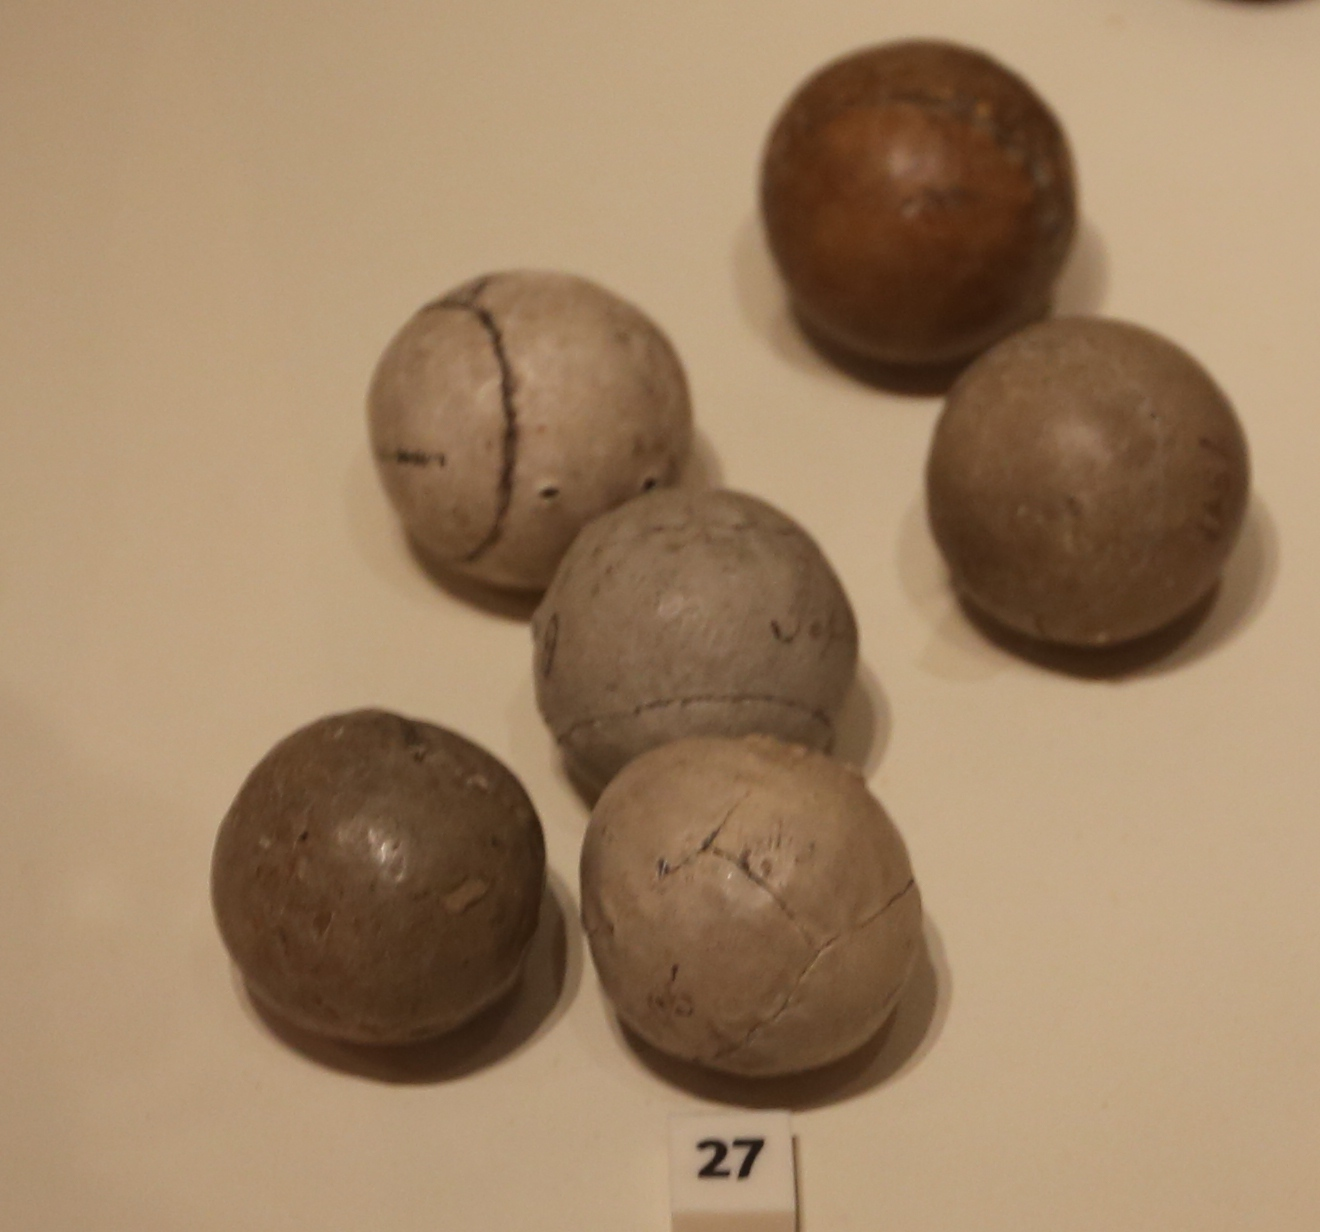
\includegraphics[scale=0.16]{../images/featherie.jpg}
\caption{``Featherie'' balls}
\label{im:featherie}
\end{subfigure}
\quad \quad \quad \quad
\begin{subfigure}[b]{0.4\textwidth}
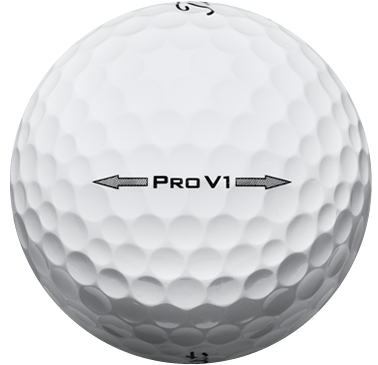
\includegraphics[scale=0.5]{../images/pv1.png}
\caption{Pro V1 ball}
\label{im:pv2}
\end{subfigure}
\caption{In \ref{im:featherie} are ``Featherie'' golf balls, taken from }
\end{figure}

After this, the golf ball once again changed form with the advent of using wrapped rubber
thread to help the ball to bounce better. This was coupled with the first time that a plastic
cover was added to the ball, in order to protect the rubber inside the ball on impact with the
club. This cover also persists to this day, although the inside of the ball has seen significant
development.

The modern golf ball has changed significantly from old designs. The interior of the ball is
now usually a 3 piece rubber composite, with different properties in each rubber to maximize
the controllability of the ball during play. The exterior is a polyurethane cover (usually white)
with usually between 300 to 400 dimples (though these can go as low as 200 dimples, and
beyond 600 in some cases). The properties of the ball are stipulated to be within certain ranges,
as set by The R\&A and USGA in the rules of golf. The weight of a ball must not be greater
than 45.93g, the diameter no less than 42.67mm and the ball must be spherically symmetric.

\chapter{Preliminary Investigations and Background}
There are some useful results we need which we'll probably write about here \citet{robinson}

\chapter{A Model of Golf Ball Flight}
This section is about \citet{Robinson2013} and the comment \citet{Jensen2014Comment} and the 
reply \citet{Robinson2014Reply}.

\section{A Model for Golf Ball Flight}

Describe the model, provide diagrams, show basic runs.

Model is a good comprimise between simplicity and flexibility. Can plug in new drag coefficents.
Some parts of the model are purely heurestic like the form for the lift, others seem just plain wrong.
The overall structure is good though. Compare basic run to data, show similar shape but incorrect
carry.

\section{Limitations of the Model}

Talk about the \citet{Jensen2014Comment} comment, dimensional analysis, lead into talking about why
we need to improve this model to find a better form for $c_{D}$. Ppotentially a way to estimate the 
spin ratio. Mention how \citet{Robinson2014Reply} addresses some of the concerns of the comment but does
not give forms for $c_{D}$. Talk about how the golf ball is in the middle between the high and low
reynold limits and this will require some matching modelling to find a good form.

\chapter{Finding $c_{d}$ and $c_{l}$}
This is where we discuss the main results we've had.

\section{Estimating $c_{D}$ from Experiments}

\begin{itemize}
\item We try to find results for spheres and change them to account for the earlier drag crisis.
\item Take the function from \citet{Morrison2010} and change the coefficents to ``move'' the drag 
drop to lower values of $Re$.
\item This works fairly well but cannot capture all of the behaviour, as other work shows that
different balls should expect to see different drags \citet{Alam2011}.
\end{itemize}

\begin{figure}[h]
\centering
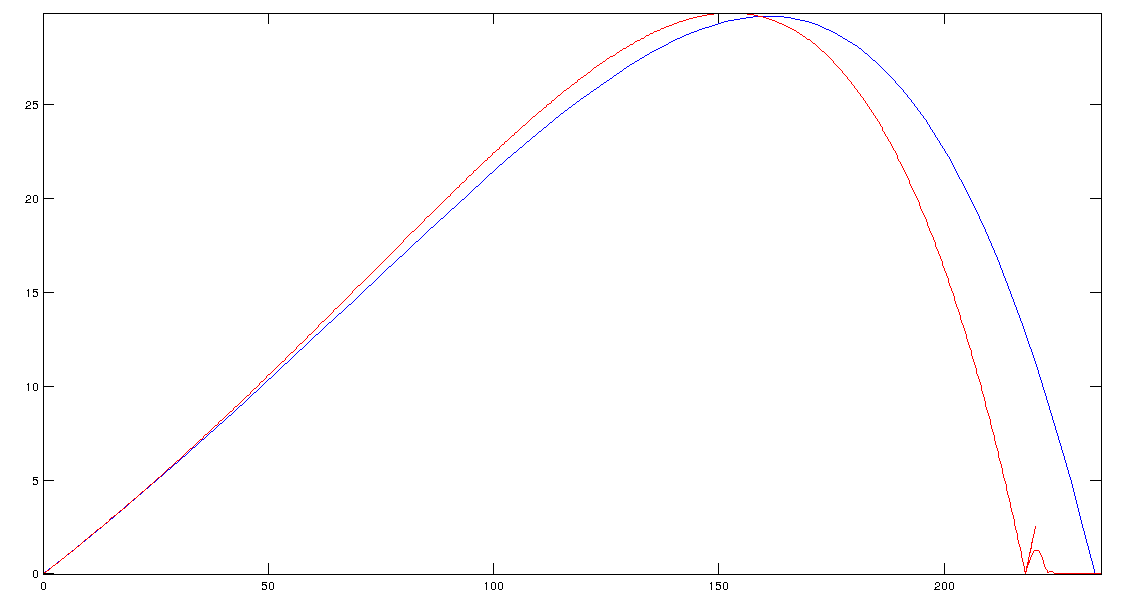
\includegraphics[scale=0.45]{../images/trajectory-older.png}
\caption[Model with $c_{D}$ dependent on $Re$.]{Using the modified Morrison form for $c_{D}$ results 
in a fairly accurate profile. Here red is the data and blue is the predictions of the model.}
\end{figure}

\begin{figure}[h]
\centering
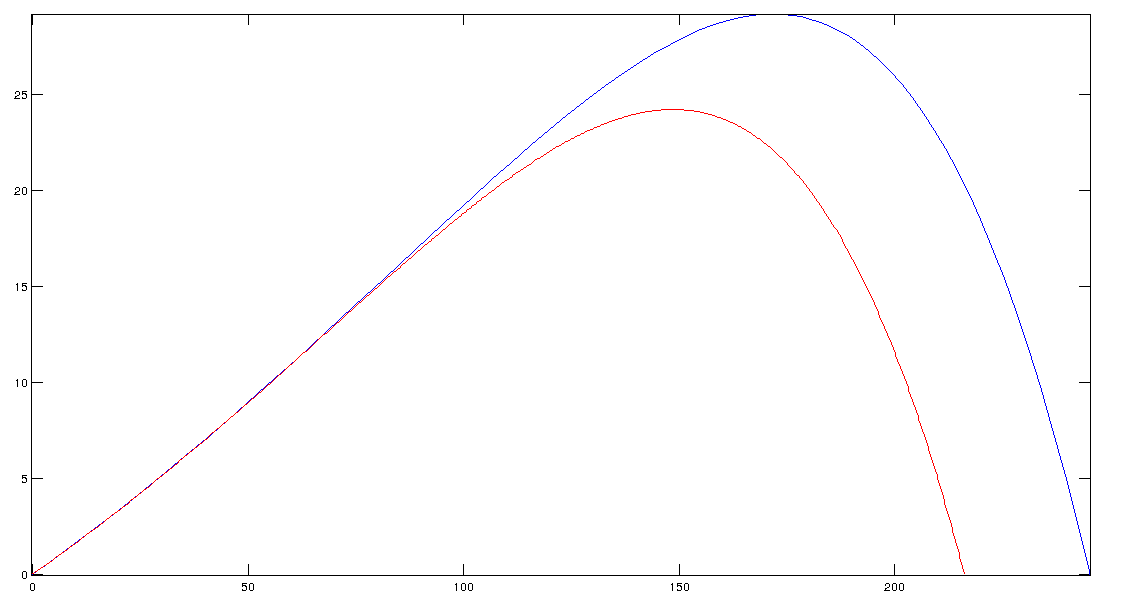
\includegraphics[scale=0.45]{../images/trajectory.png}
\caption[Second data set with Morrison drag.]{The Morrison drag form does not always produce accurate
results, however we do see good agreement at the start. Here red is the data and blue is the 
predictions of the model.}
\end{figure}

\section{Parameterising $c_{D}$ and $c_{L}$ by Non Dimensional Variables}

\begin{itemize}
\item We follow the idea from \citet{Lieberman2001}: form $c_{D}$ and $c_{L}$ from dimensionless
groupings and use the data to estimate the parameters in this model.
\item Use least squares to do this. See Appendix for discussion of what an inverse problem is, how
to use least squares to solve them, and what numerical techniques there are to do this.
\item Find that doing this is very hard: the problem is likely not well posed and finding a minimum
is difficult. Would benefit from a more through analysis of the least squares problem but unsure how
this would be done.
\item This inverse problem is a good way to move forwards with the problem in the future.
\end{itemize}

\section{$\tanh$ Matching}

\begin{itemize}
\item Take a hybrid approch between the two previous ideas: form a function which ``looks'' similar
to \citet{Morrison2010} and has the same behaviour, but is parameterised in such a way as to allow
us to use a least squares solver to estimate parameters.
\item For the drop, use a $\tanh$ function of the form
\[
c_{D} = a + b \tanh (-c(Re - d))
\]
where $a,b,c,d$ are constants which we can use least squreas to determine.
\item Match the $\tanh$ at the top with the $24/Re$ form we know from spheres and past the drop match
to the weakly linear form we see from the previous work.
\item Still trying to decide on results for this.
\end{itemize}

% \chapter{Some new theorems that give rise to a very long chapter name}
% \chaptermark{Shortened chapter header}

% % Comment the following THREE lines if you do NOT have an Appendix
% \appendix
% \chapter{A Long Proof}
% .........

% % If you need more than one appendix, then just use another \chapter command
% %\chapter{Yet Another Appendix}

\bibliography{Golf-CFD,Golf-physics,Inverse_Problems}

\end{document}
